% Figure 5 composite (vector). Build: pdflatex fig5_assemble.tex
\documentclass[tikz,border=1mm]{standalone}
\usepackage{graphicx}\usepackage{helvet}\renewcommand{\familydefault}{\sfdefault}
\begin{document}
\begin{tikzpicture}[x=1mm,y=1mm]
  \useasboundingbox (0,0) rectangle (183,150);
  % row 1: a oracle def (AI) | b oracle vs model | c phase map
  \node[anchor=north west,inner sep=0] at (4,146)  {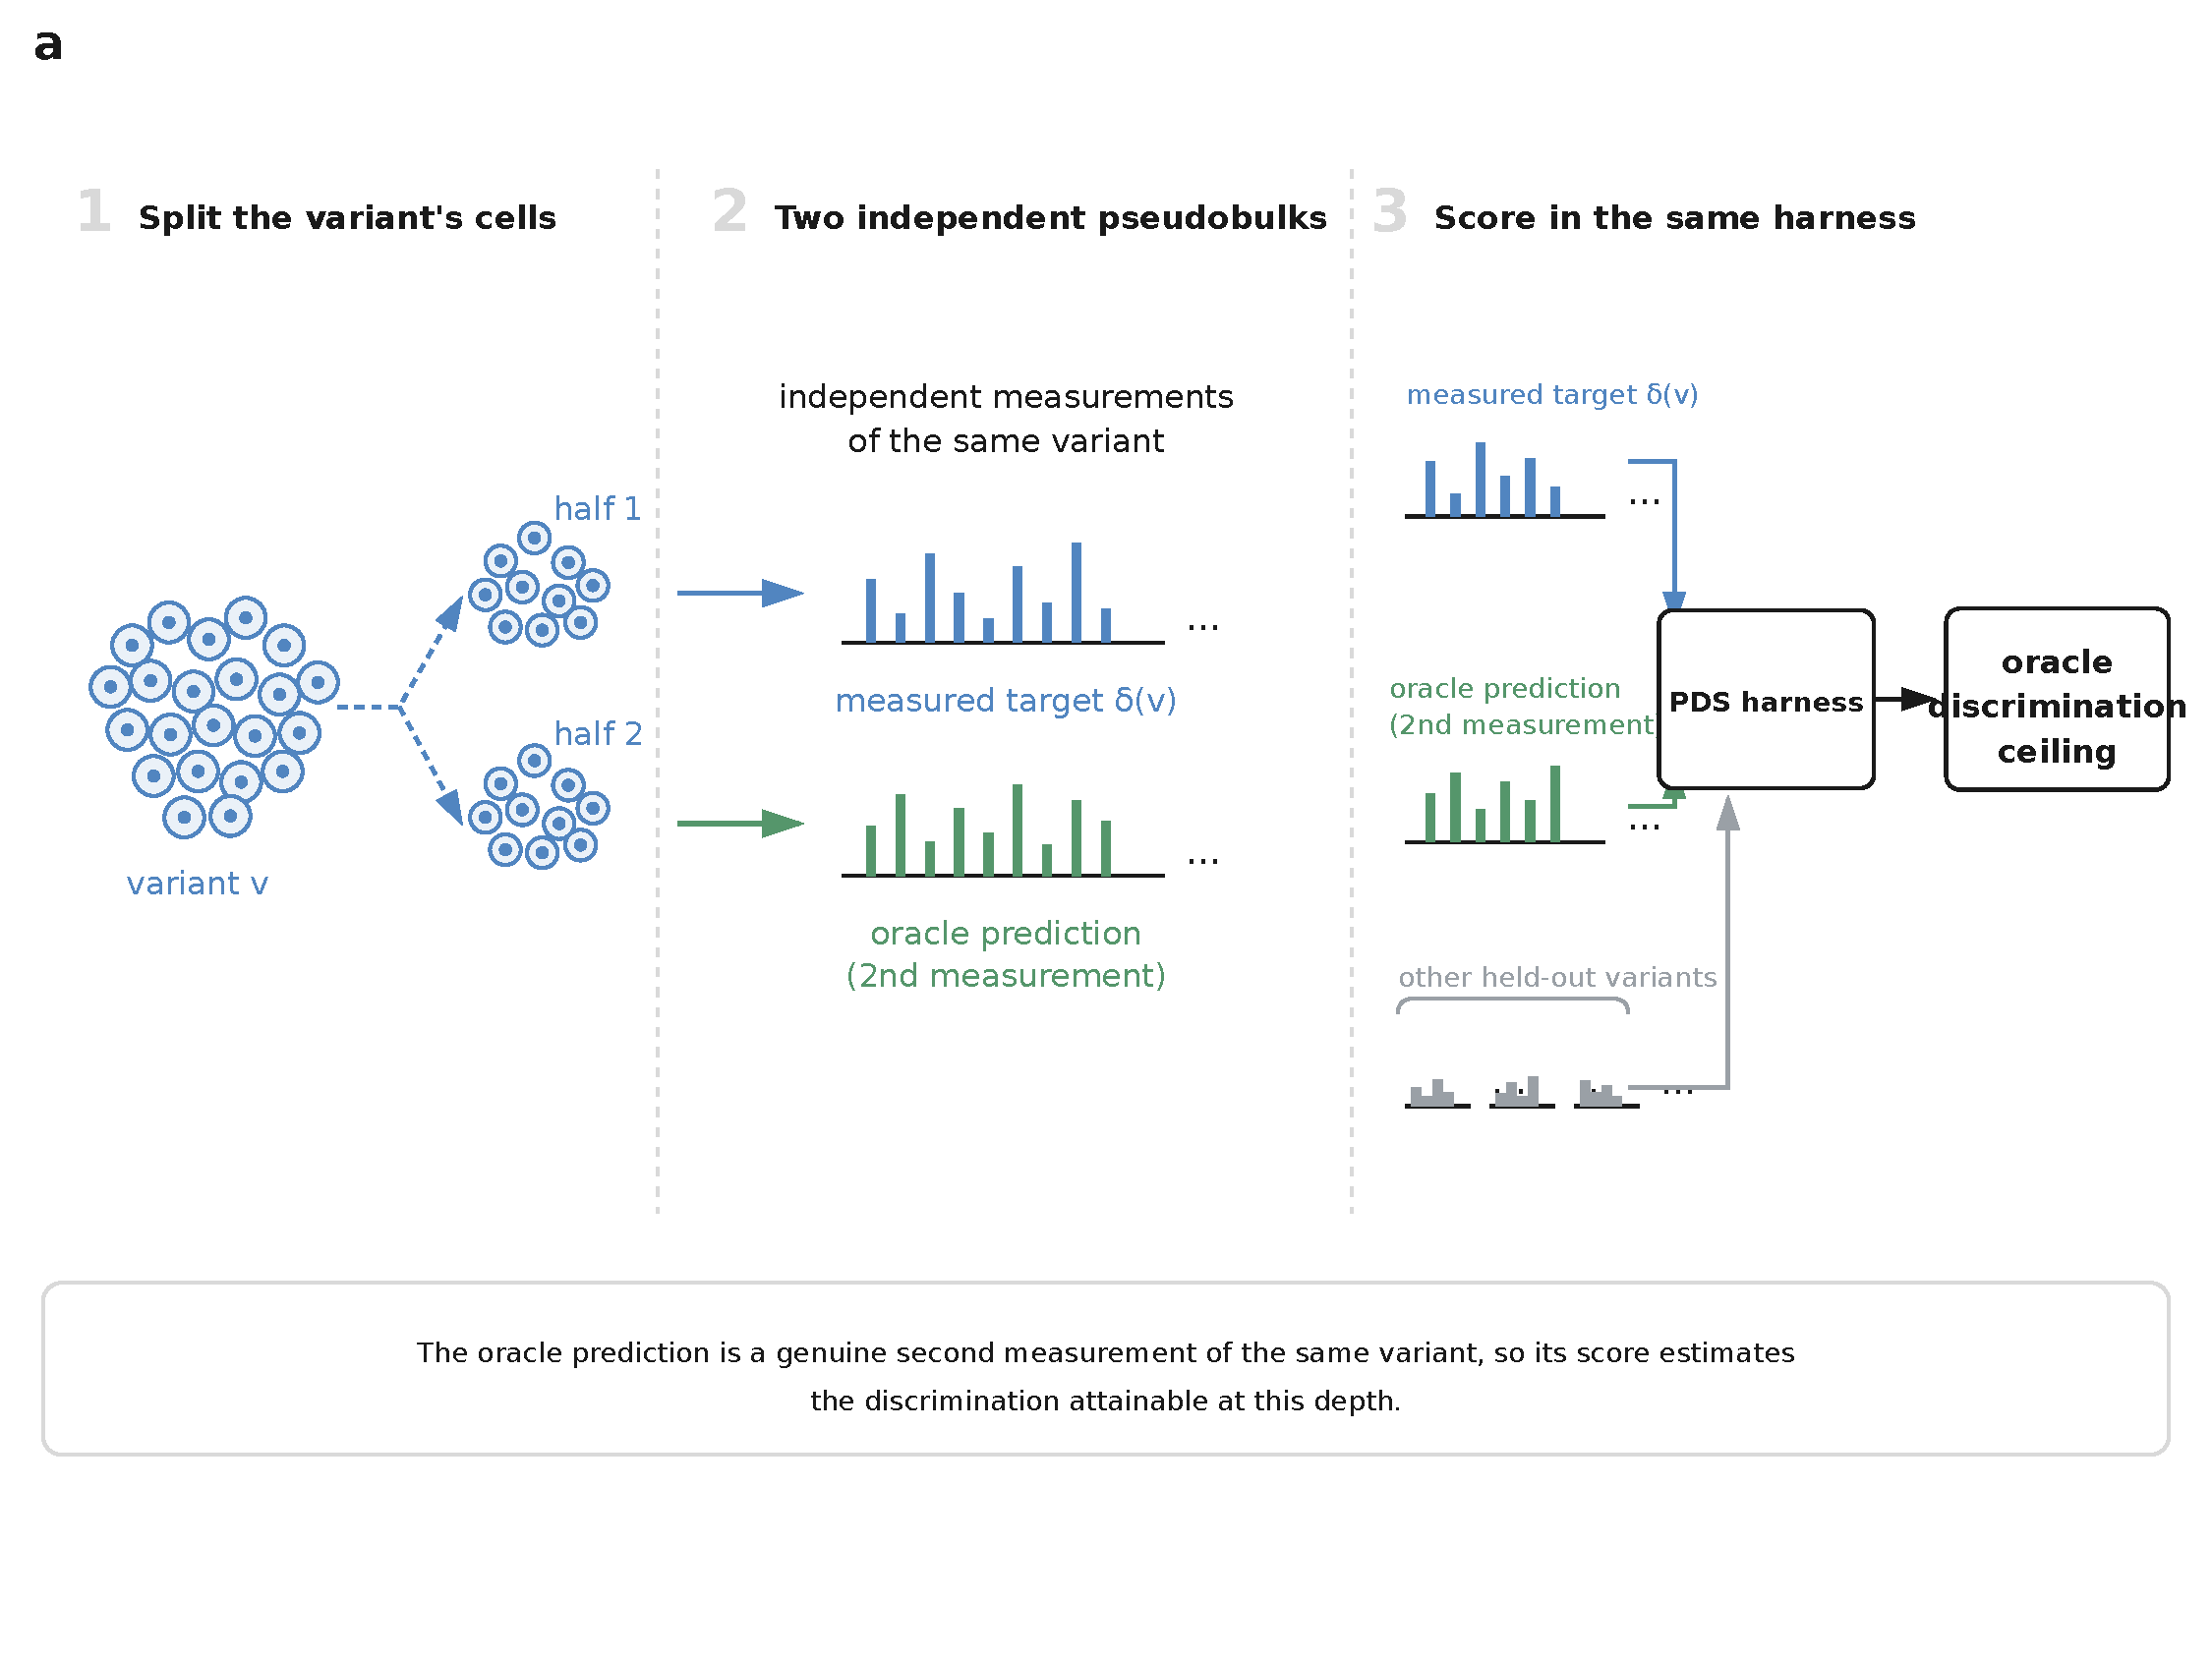
\includegraphics[width=60mm]{Fig5a_oracle_ceiling.pdf}};
  \node[anchor=north west,inner sep=0] at (68,146) {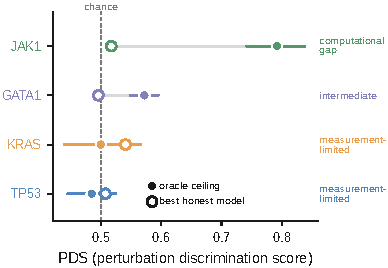
\includegraphics[width=58mm]{fig5b_oracle_vs_model.pdf}};
  \node[anchor=north west,inner sep=0] at (130,146){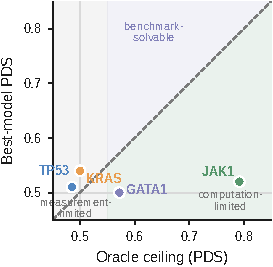
\includegraphics[width=44mm]{fig5c_phasemap.pdf}};
  % row 2: d synthetic predictors (AI) | e leaderboard example (AI) | f resolution curve
  \node[anchor=north west,inner sep=0] at (4,98)   {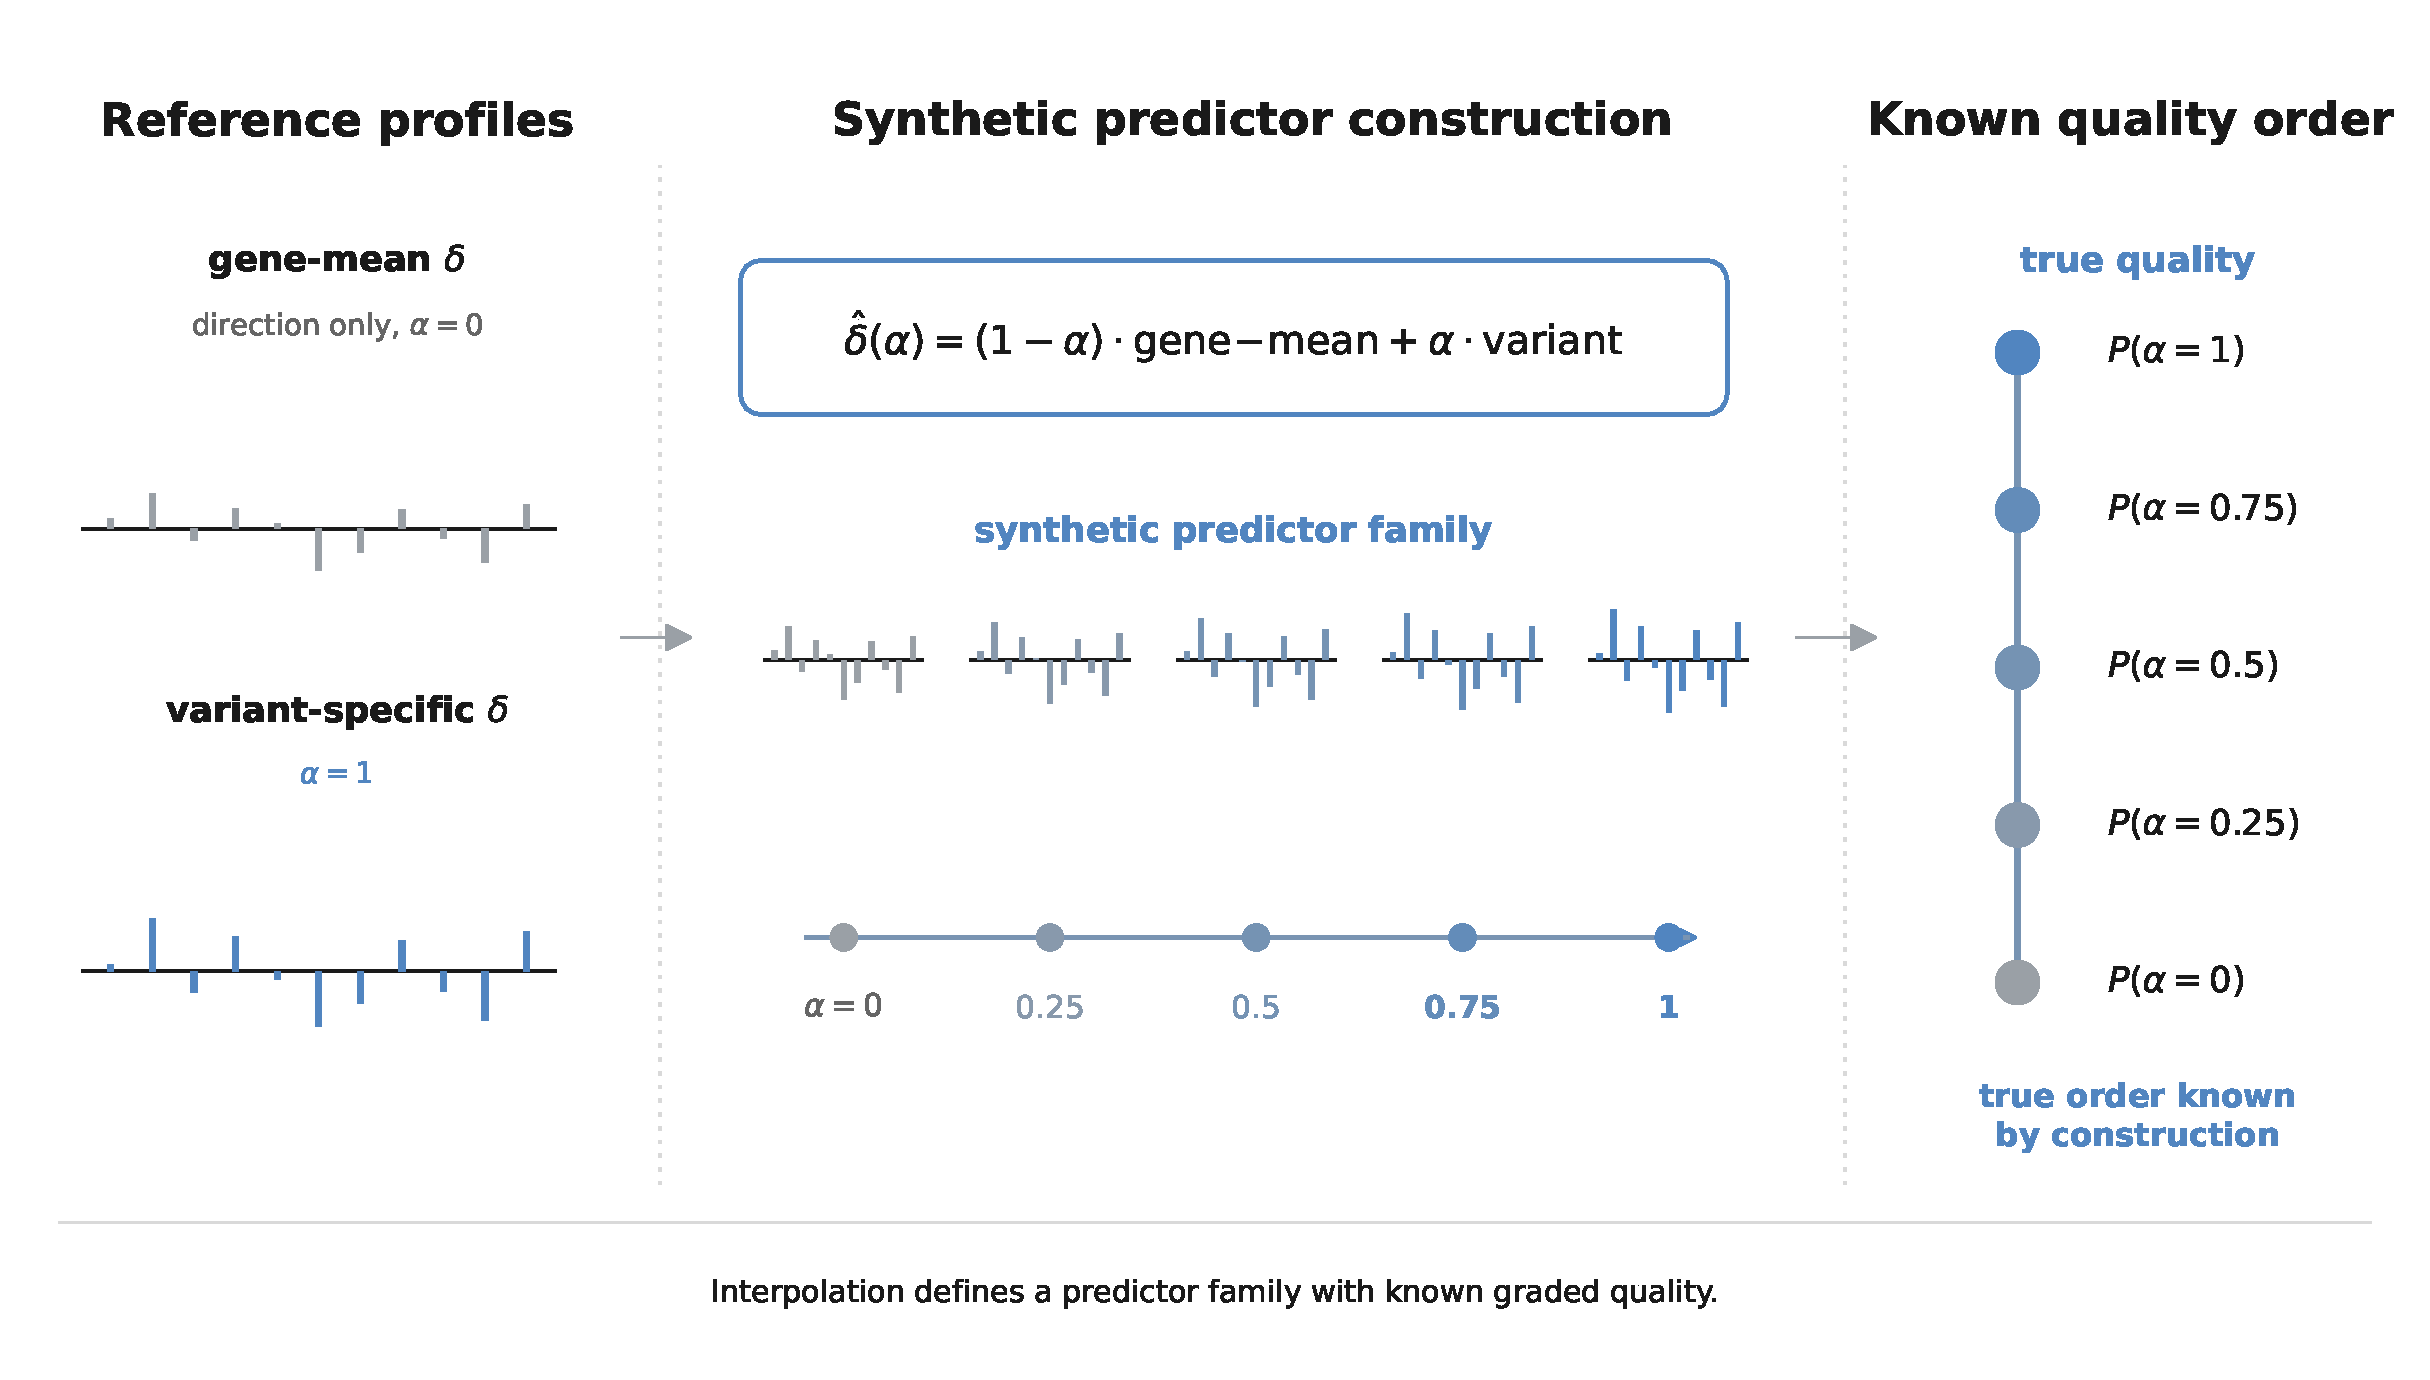
\includegraphics[width=60mm]{Fig5d.pdf}};
  \node[anchor=north west,inner sep=0] at (68,98)  {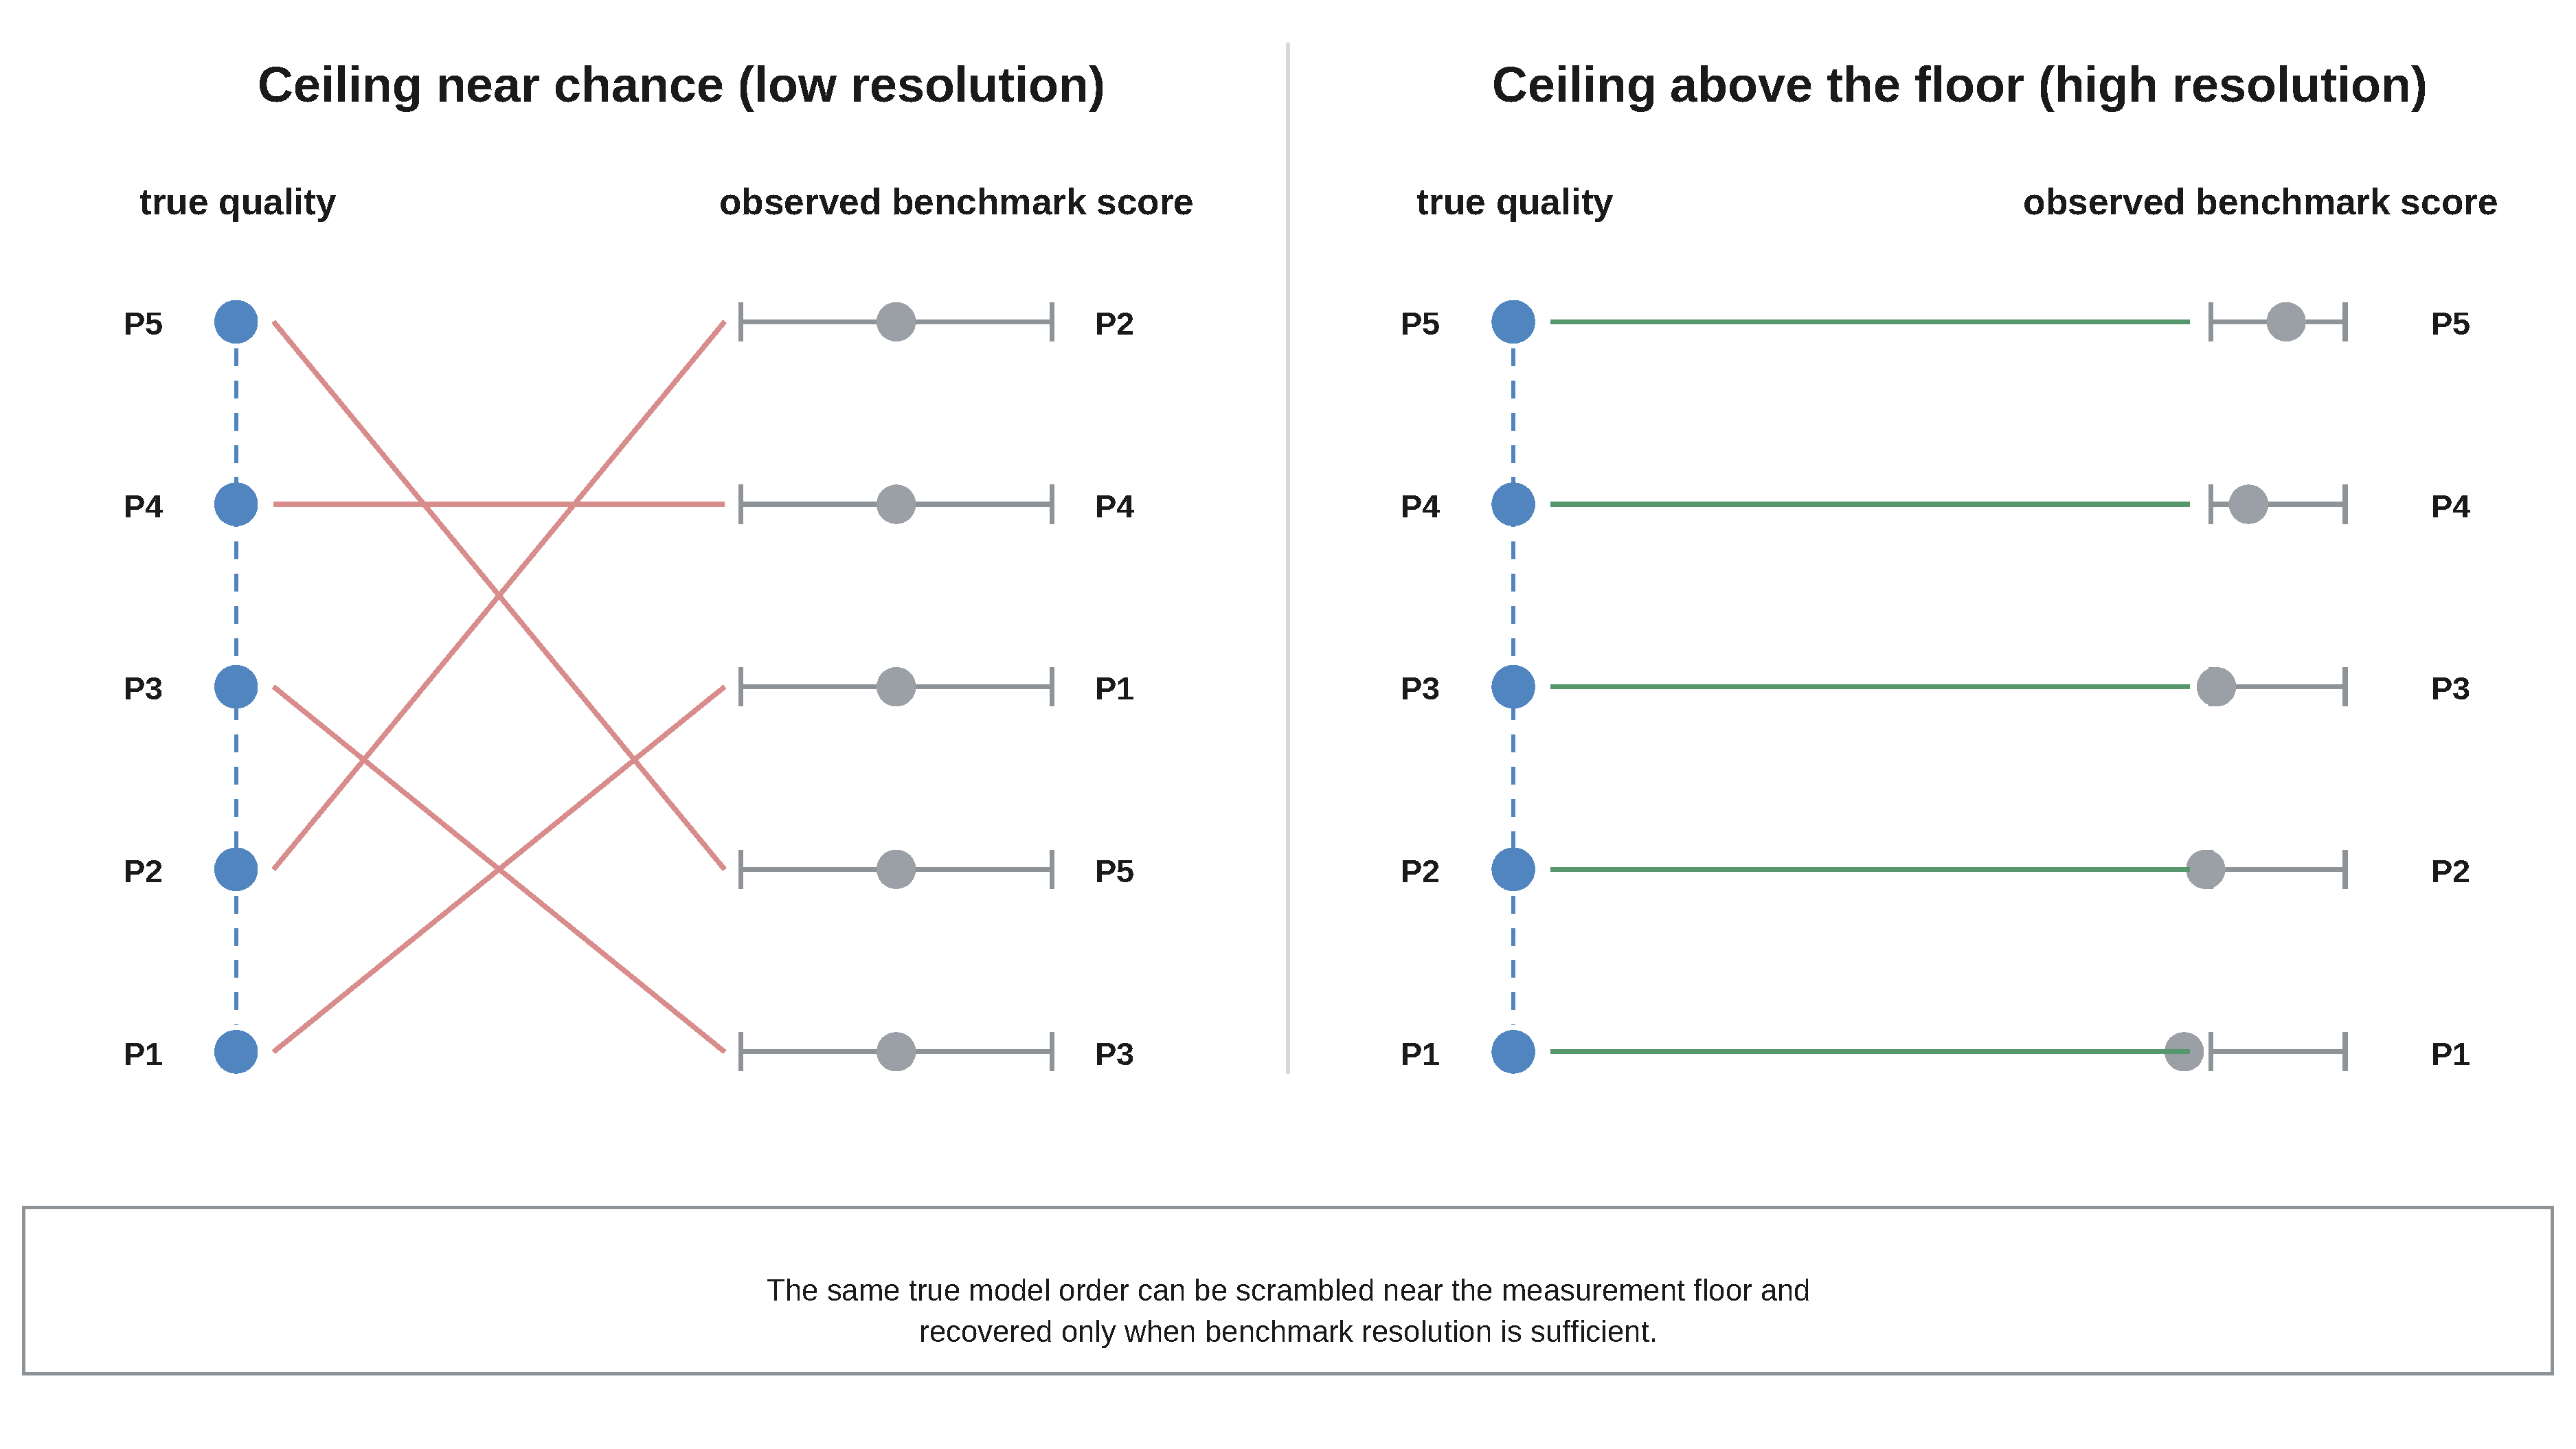
\includegraphics[width=58mm]{Fig5e.pdf}};
  \node[anchor=north west,inner sep=0] at (128,98) {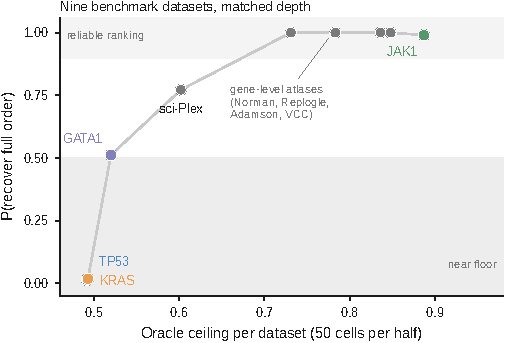
\includegraphics[width=54mm]{fig5f_resolution.pdf}};
  % row 3: g benchmark-validity transition
  \node[anchor=north west,inner sep=0] at (48,62)  {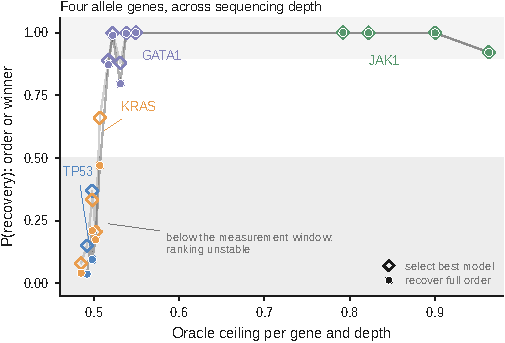
\includegraphics[width=90mm]{fig5g_validity.pdf}};
  % panel letters
  \tikzset{plab/.style={font=\bfseries\large,anchor=north west,inner sep=0}}
  \node[plab] at (1,149) {a};  \node[plab] at (65,149) {b};  \node[plab] at (127,149) {c};
  \node[plab] at (1,101) {d};  \node[plab] at (65,101) {e};  \node[plab] at (125,101) {f};
  \node[plab] at (45,65) {g};
\end{tikzpicture}
\end{document}
